\chapter{Scope, Questions, and Review Method}
\label{ch:scope}

\section{What this manuscript reviews}

The repository combines three artifact classes that require different tests:

\begin{enumerate}
  \item established mathematical constructions and their implementations;
  \item numerical experiments that test algorithms or dynamical models; and
  \item physical interpretations proposed in source manuscripts.
\end{enumerate}

The classes are related, but they are not interchangeable. A correct Cartan
matrix does not validate a fluid model. A stable numerical trajectory does not
prove a theorem. A dimensional identity does not establish a new interaction.
The review treats every transition between classes as a separate claim that
needs its own argument and evidence.

\section{Questions}

The audit asks four questions.

\begin{description}
  \item[Definition] Is the mathematical or physical object defined well enough
    to determine what would count as an error?
  \item[Derivation] Does the conclusion follow from the premises, with all
    additional assumptions stated?
  \item[Reproduction] Can the reported computation be regenerated from a named
    program, parameter set, and retained output?
  \item[Falsification] What observation or controlled comparison would reject
    the proposed physical interpretation?
\end{description}

These questions are intentionally conservative. They do not ask whether a
cross-domain analogy is interesting. They ask whether the analogy has been
promoted to a mechanism without the work needed to justify that promotion.

\section{Evidence vocabulary}

The earlier manuscript used terms such as \enquote{verified}, \enquote{proved},
and \enquote{confirmed} for several incompatible kinds of support. This edition
uses the following controlled vocabulary.

\begin{table}[htbp]
  \centering
  \caption{Evidence classes used throughout the review.}
  \label{tab:evidence-classes}
  \begin{tabularx}{\textwidth}{>{\raggedright\arraybackslash\bfseries}p{0.20\textwidth}Y}
    \toprule
    Class & Required support \\
    \midrule
    Established result & A theorem or standard result with a suitable source. \\
    Source claim & A statement found in the reviewed corpus, with no implied endorsement. \\
    Computational check & A program and retained output that test a specified finite case. \\
    Hypothesis & A proposed relation with a stated test and possible failure outcome. \\
    Unsupported extrapolation & A conclusion for which the repository supplies no valid derivation or discriminating evidence. \\
    Invalid artifact & An output that is malformed or fails a prerequisite numerical check. \\
    \bottomrule
  \end{tabularx}
\end{table}

\section{Evidence surfaces}

The review uses repository paths as provenance locators. The principal
surfaces are:

\begin{itemize}
  \item \texttt{papers/references.bib}, for bibliographic records;
  \item \texttt{source\_materials/pdfs/}, for retained source documents;
  \item \texttt{src/mathphysics/}, for reusable implementations;
  \item \texttt{experiments/}, for experiment drivers and retained JSON output;
  \item \texttt{results/}, for retained simulation snapshots; and
  \item \texttt{data/registry/}, for generated indexes and integrity metadata.
\end{itemize}

Registry presence establishes identity and lineage, not scientific validity.
A SHA-256 digest can show that an artifact has not changed; it cannot show that
the method that produced it was correct.

\section{Claim-to-evidence protocol}

Each physical claim is evaluated in the same order:

\begin{enumerate}
  \item state the source claim without strengthening it;
  \item identify the standard mathematics or physics it invokes;
  \item isolate the extra step needed to reach the claimed conclusion;
  \item inspect the repository for an implementation or measurement of that
    extra step; and
  \item record the strongest conclusion the available evidence permits.
\end{enumerate}

This ordering prevents a common failure mode in speculative synthesis: a
correct premise is presented, an analogy is inserted, and the final conclusion
inherits the authority of the premise despite not following from it.

\begin{figure}[htbp]
  \centering
  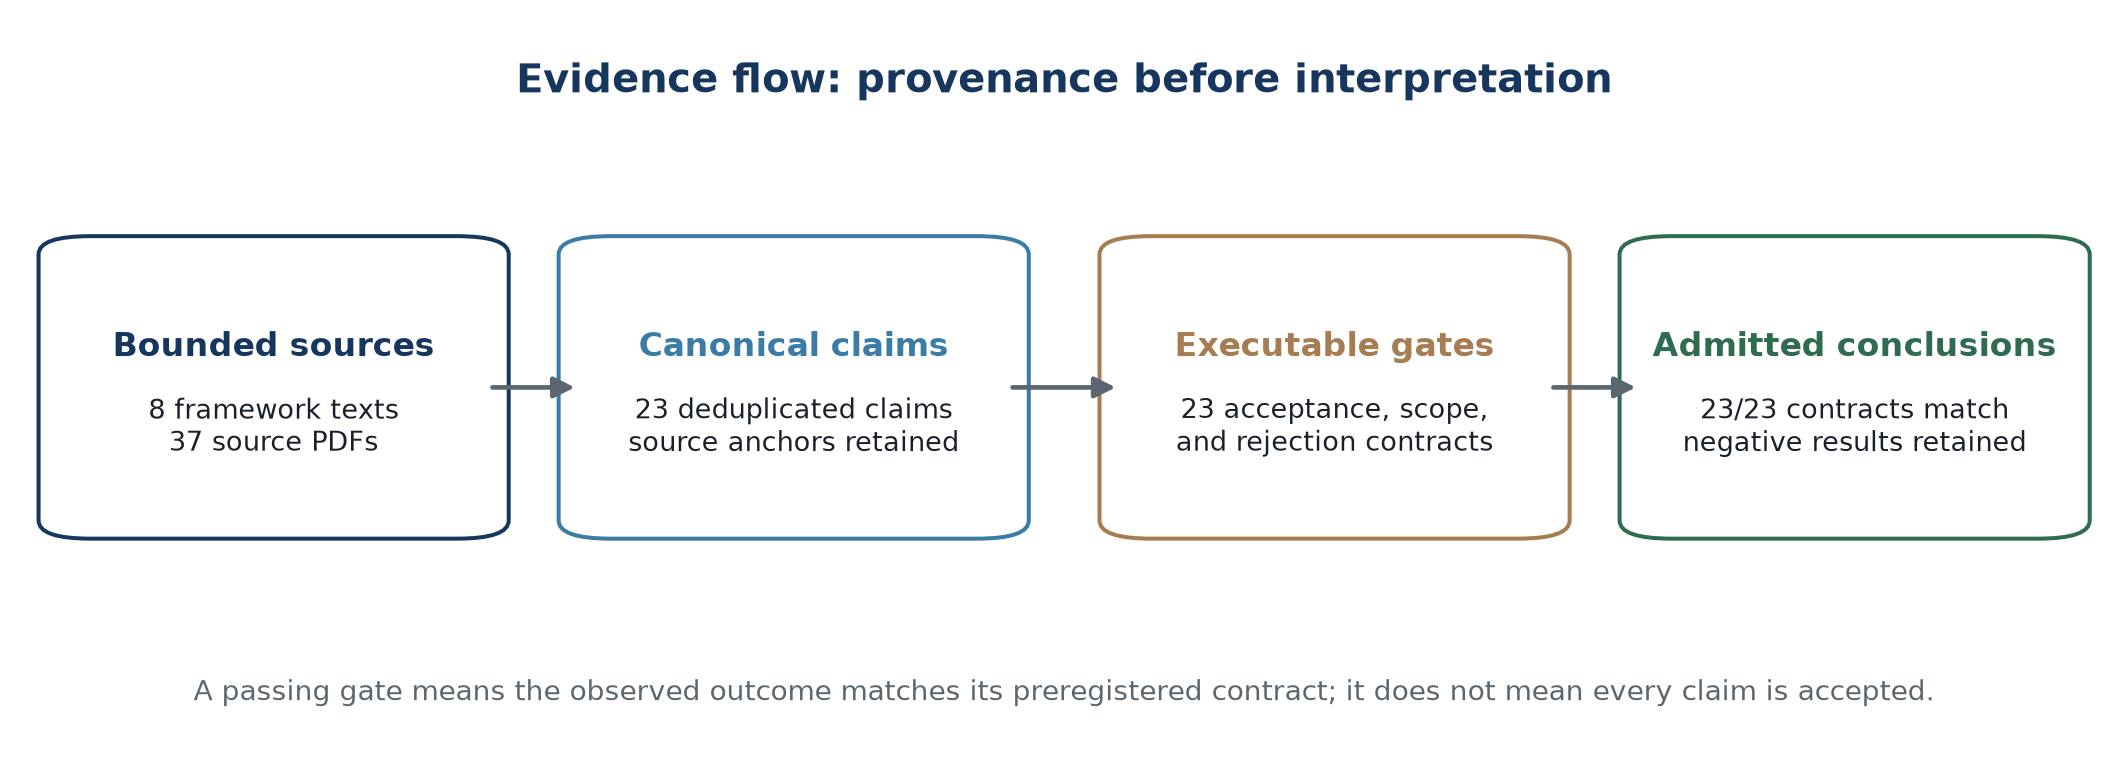
\includegraphics[width=\textwidth]{figures/review_evidence_flow.png}
  \caption{The evidence pipeline separates source provenance, canonical claims,
  executable gates, and admitted conclusions. A passing gate may preserve a
  falsification or exclusion result.}
  \label{fig:evidence-flow}
\end{figure}

\section{Canonical claim disposition}

The unified ledger contains 23 claims. Each has exactly one executable gate,
and the generated result records whether the observed outcome matches the
declared status and rejection contract.

\begin{figure}[htbp]
  \centering
  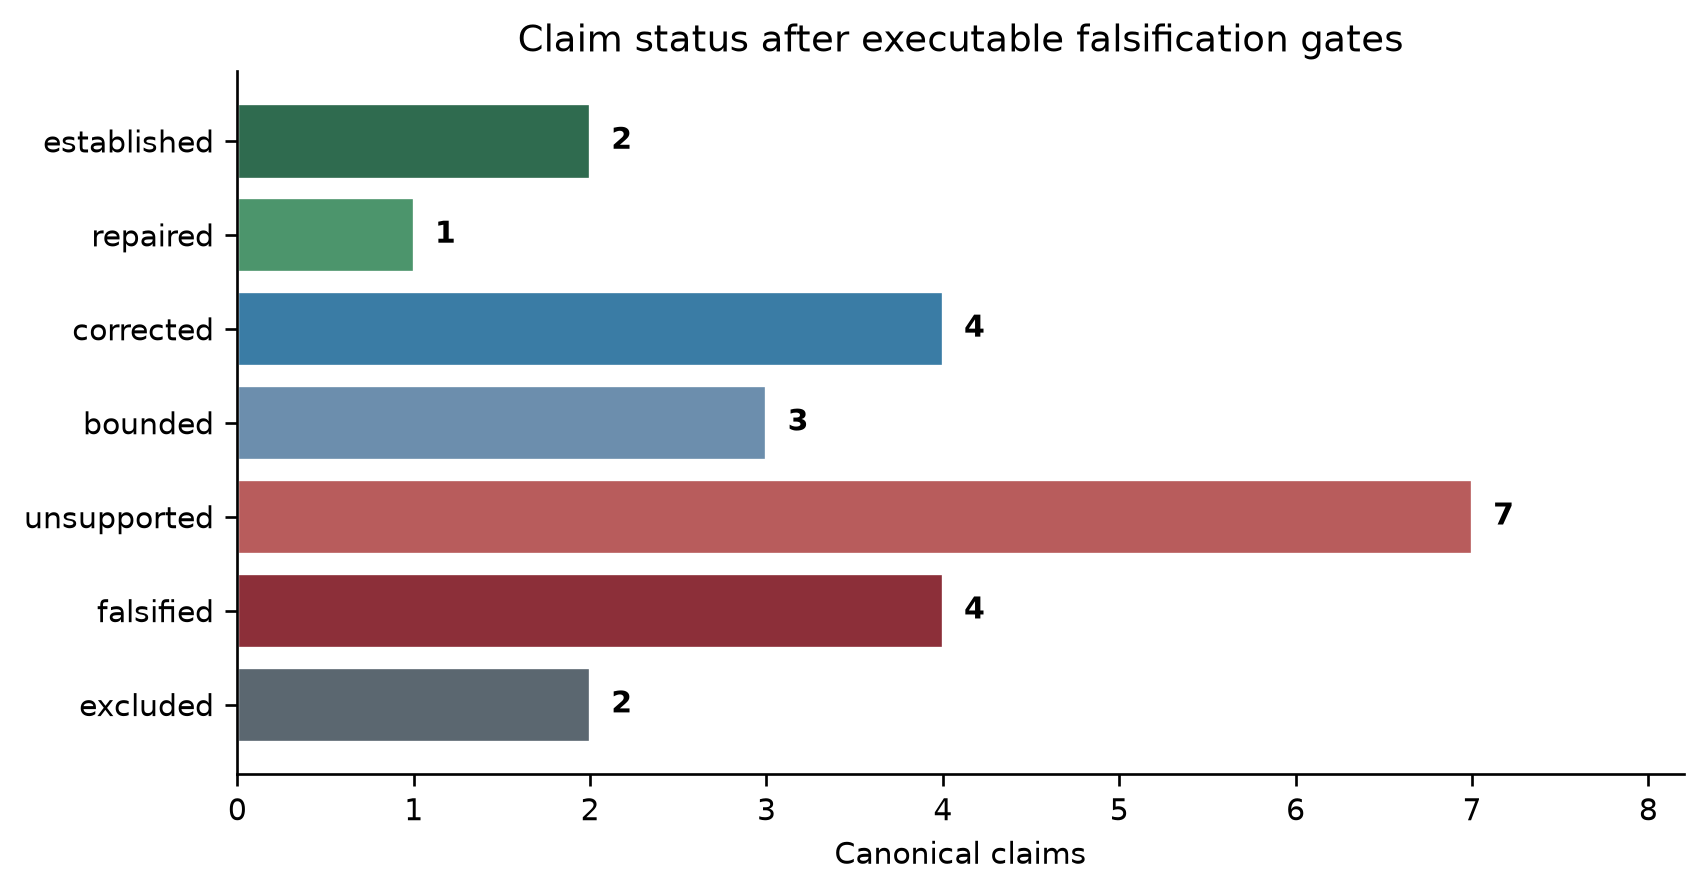
\includegraphics[width=0.82\textwidth]{figures/review_claim_status.png}
  \caption{Claim statuses after mathematical, computational, scope, and
  measurability gates.}
  \label{fig:claim-status}
\end{figure}

\small
\begin{longtable}{>{\raggedright\arraybackslash}p{0.36\textwidth}
                  >{\raggedright\arraybackslash}p{0.16\textwidth}
                  >{\raggedright\arraybackslash}p{0.14\textwidth}
                  >{\raggedright\arraybackslash}p{0.13\textwidth}}
  \caption{Canonical claim status and executable gate outcome.}
  \label{tab:claim-status}\\
  \toprule
  Claim & Domain & Claim status & Gate outcome \\
  \midrule
  \endfirsthead
  \toprule
  Claim & Domain & Claim status & Gate outcome \\
  \midrule
  \endhead
  Octonion normed division boundary & Nonassociative algebra & established & accepted \\
Higher Cayley Dickson physical mapping & Mathematical physics & unsupported & rejected \\
Albert exceptional group ladder & Jordan algebra & corrected & corrected \\
Spin8 triality & Lie theory & established & accepted \\
E9 E10 E11 classification & Kac Moody algebra & corrected & corrected \\
E10 E11 supergravity scope & Quantum gravity & bounded & bounded \\
Monstrous moonshine stability & Modular forms & unsupported & rejected \\
Fractional and negative dimension scope & Fractal geometry & corrected & corrected \\
Fractal estimator convergence & Numerical analysis & bounded & bounded \\
Scalar field curvature mechanism & Field theory & unsupported & rejected \\
ZPE energy harvesting & Quantum field theory & unsupported & rejected \\
Time crystal energy amplification & Condensed matter physics & unsupported & rejected \\
Planck force unification & Dimensional analysis & unsupported & rejected \\
Origami fold merge operator & Operator theory & excluded & excluded \\
E7 root quotient charge & Lattice theory & falsified & falsified \\
External Fourier quotient map & Lattice theory & falsified & falsified \\
Kac Moody fluid transfer & Mathematical physics & unsupported & rejected \\
LBM beta plane and jets & Computational fluid dynamics & falsified & falsified \\
Matched beta plane algebraic ablation & Computational fluid dynamics & falsified & falsified \\
LBM equilibrium conservation & Computational fluid dynamics & repaired & repaired \\
Tourmaline novel energy effect & Materials science & bounded & bounded \\
Gravitoelectromagnetism scope & General relativity & corrected & corrected \\
Consciousness resonance & Biophysics & excluded & excluded \\
\bottomrule

\end{longtable}
\normalsize

\section{Limits of this review}

The review does not independently reproduce every theorem cited in the corpus,
nor does it treat repository tests as substitutes for peer review. It evaluates
what the checked-in artifacts can support. Claims that require laboratory data,
hardware execution, or a new mathematical proof remain open only when the
claim is defined precisely enough to test. Otherwise they remain unsupported,
not merely unfinished.

The beta-plane study is a short, decaying, periodic-domain implementation test;
it does not establish statistically stationary turbulence or persistent jets.
The algebra audits combine literature scope with exact counterexamples and
finite numerical residuals; sampled identities do not replace universal proofs.
No new materials, vacuum-energy, time-crystal-energy, gravitational, or
biophysical experiment was performed. Those claims therefore remain bounded,
rejected, or excluded according to their admission packages rather than being
promoted by the breadth of the source corpus.
